\documentclass[tikz,multi,border=10pt]{standalone}
\usetikzlibrary{shadows,arrows.meta,positioning,backgrounds,fit}

% Define block styles
\tikzset{%
  materia/.style={draw, fill=blue!20, text width=6.0em, text centered, minimum height=1.5em,drop shadow},
  etape/.style={materia, text width=8em, minimum width=10em, minimum height=3em, rounded corners, drop shadow},
  texto/.style={above, text width=6em, text centered},
  linepart/.style={draw, thick, color=black!50, -LaTeX, dashed},
  line/.style={draw, thick, color=black!50, -LaTeX},
  ur/.style={draw, text centered, minimum height=0.01em},
  back group/.style={fill=yellow!20,rounded corners, draw=black!50, dashed, inner xsep=15pt, inner ysep=10pt},
}

\newcommand{\etape}[2]{node (p#1) [etape] {#2}}

\newcommand{\transreceptor}[3]{%
  \path [linepart] (#1.east) -- node [above] {\scriptsize #2} (#3);}

\begin{document}
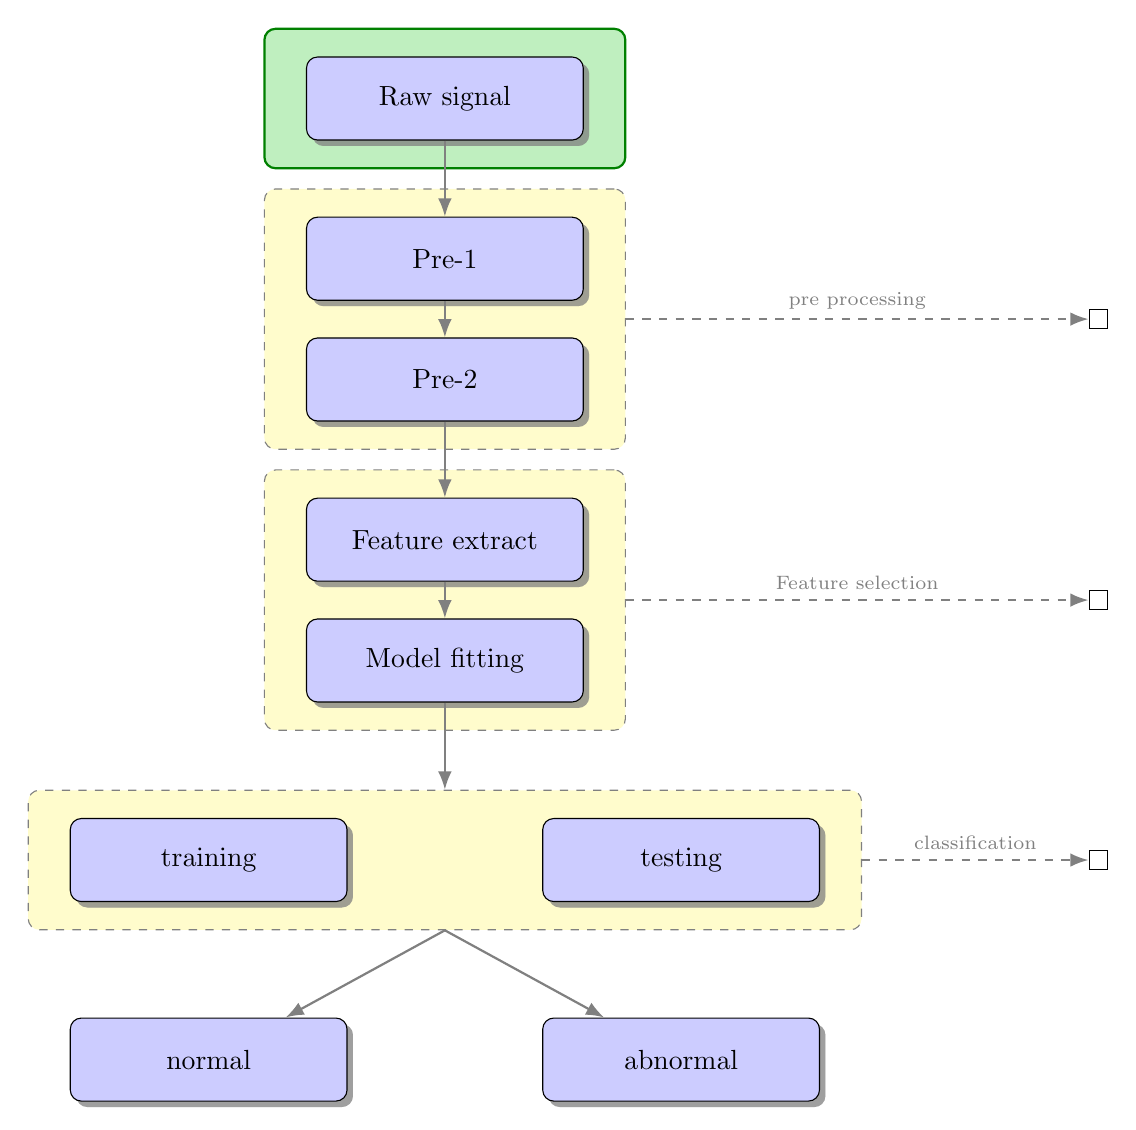
\begin{tikzpicture}

  % Draw diagram elements
  \path \etape{1}{Raw signal};

  \path (p1.south)+(0.0,-1.5) \etape{2}{Pre-1};
  \path (p2.south)+(0.0,-1.0) \etape{3}{Pre-2};

  \path (p3.south)+(0.0,-1.5) \etape{4}{Feature extract};
  \path (p4.south)+(0.0,-1.0) \etape{5}{Model fitting};

  \path (p5.south)+(-3.0,-2.0) \etape{6}{training};
  \path (p5.south)+(3.0,-2.0) \etape{7}{testing};
  \node [below=of p5] (p6-7) {};

  \path (p6.south)+(0.0,-2.0) \etape{8}{normal};
  \path (p7.south)+(0.0,-2.0) \etape{9}{abnormal};
  \node [below=of p6-7] (p8-9) {};

  % Draw arrows between elements
  \path [line] (p1.south) -- node [above] {} (p2);
  \path [line] (p2.south) -- node [above] {} (p3);
  \path [line] (p3.south) -- node [above] {} (p4);
  \path [line] (p4.south) -- node [above] {} (p5);

  \begin{scope}[on background layer]
    \node (bk1) [back group] [fit=(p2) (p3)] {};
    \node (bk2) [back group] [fit=(p4) (p5)] {};
    \node (bk3) [back group] [fit=(p6) (p7)] {};
    \node [draw, thick, green!50!black, fill=green!75!black!25, rounded corners, fit=(p1), inner xsep=15pt, inner ysep=10pt] {};
  \end{scope}

  \path [line] (p5.south) -- node [above] {} (bk3.north);
  \path [line] (bk3.south) -- node [above] {} (p8);
  \path [line] (bk3.south) -- node [above] {} (p9);
  \path (bk1.east)+(+6.0,0) node (ur1)[ur] {};
  \path (bk2.east)+(+6.0,0) node (ur2)[ur] {};
  \path (bk3.east)+(+3.0,0) node (ur3)[ur] {};
  \transreceptor{bk1}{pre processing}{ur1};
  \transreceptor{bk2}{Feature selection}{ur2};
  \transreceptor{bk3}{classification}{ur3};
\end{tikzpicture}
\end{document}
